% !TEX root =  ../main.tex
\chapter{Synthèse d'un régulateur continu}

\section{Introduction}
Durant cette seconde séance de laboratoire, il a été demandé aux étudiants de synthétiser sur le logiciel MATLAB un régulateur continu en boucle fermée.
Une fois cette étape réalisée, la discrétisation de ce régulateur selon 3 périodes d'échantillonnage a été effectuée afin d'obtenir 3 régulateurs discrets.
Le but final était alors de comparer, grâce à Simulink, les performances du régulateur continu avec les 3 régulateurs discrets obtenus. 

\section{Notions théoriques}


\section{Analyse}
Nous avons construit un régulateur continu par cancelation des poles et zeros en gardant l'intégrateur.
Dans la chaine direct il reste un simple intégrateur avec un simple gain qu'il faut determiner.
Quand on reboucle un intégrateur avec un simple gain on a un filtre du premier ordre donc ça permet de placer la constante de temps.

On synthétise le régulateur continu et puis on discrétise.
L'inconvénient de cette procedure est qu'on n'a pas pris en compte le bloqueur d'ordre 0.
Ce bloqueur en moyenne entraine un retard d'une demi période.
Cela veut dire que cela fera tomber la courbe des phases et qu'on pourra partir en instabilité à un moment.
Plus la période d'échantillonnage est grande plus cela se dégrade.
On fait le passage continu discret du régulateur par les différences finies à gauche et on sait qu'avec les pôles dans le plan gauche, on peut avoir une projection a l'extérieur du cercle.
Donc des pôles stables continus peuvent devenir instables en discret. Ce sont les inconvénients de la méthode.

La deuxième étape était de discrétiser le système par l'équivalent échantillonné bloqué.
Cela veut dire qu'on passe du domaine S vers Z en tenant compte du bloqueur et qu'on réalise une vraie synthèse discrète de la même façon en prenant les pôles du système pour les mettre aux zeros du régulateur et inversement.
On maintient l'intégrateur discret avec le dénominateur. 
Et on reboucle pour aller placer les poles discrets à l'endroit voulu c'est à dire les poles continus projetés en Z avec $Z=e^{sh}$.

Quand on discrétise par les différences finies à gauche, la réponse du système souhaité et celle qu'on obtient sont quasiment les mêmes quand la période d'échantillonnage est petite et que le temps mort supplémentaire ne nous embête pas trop.

La vraie synthèse discrète est lorsque le système est discrétisé avec c2d et là on a que la réponse est exactement celle qu'on souhaite.

Avec la discrétisation du régulateur, on commence à avoir des problèmes car on ne tient pas compte du bloqueur.

Dans le dernier cas, aux instants d'échantillonnage, on est sur la valeur souhaitée. En dehors de ces instants, on ne maitrise pas car on a imposé les pôles d'un système discret pour qu'aux instants d'échantillonnage on soit sur la réponse du filtre du premier ordre.
La réponse souhaitée est la réponse avec un régulateur synthétisé en continu et discrétisé et donc on n'a pas tenu compte dans la synthèse du régulateur du bloqueur d'ordre 0.


\section{Manipulations}
\subsection{Synthétiser le régulateur continu}
On a la fonction transfert :\\

$$H(s) = \frac{7(s+1))}{s(3s+1)}$$

Il faut synthétiser un régulateur continu tel que :
\begin{itemize}
    \item Il n'y ai pas de dépassement
    \item Le temps de réponse à 95pc soit égal à 5.
\end{itemize}

On va simplement concevoir un régulateur de compensation en simplifiant les pôles et les zéros tout en conservant notre intégrateur :\\


$$R(s) = \frac{(3s+1))}{(s+1)}.\frac{K}{7}$$


On peut calculer le gain K comme on connait le temps de réponse à 95pc :\\


$$3T = 5$$
$$T = \frac{5}{3} = \frac{1}{K}$$ 
$$K = \frac{3}{5}$$



\subsection{Discrétiser le régulateur}
pour discrétiser le régulateur on utilise la méthode des différences finies à gauche en posant :\\

$$s = \frac{z - 1}{h}$$


Ce qui donne :

$$R(z) = \frac{3z - 3 + h}{z - 1 + h}.\frac{3}{35}$$

On doit calculer les régulateurs discrétisés aux périodes d'échantillonnages suivantes :
\begin{itemize}
    \item h = 0.01 (1)
    \item h = 0.5 (2)
    \item h = 2 (3)
\end{itemize}

Pour discrétisé dans matlab on utilise, la fonction c2d à qui on donne le régulateur continu et la période d'échantillonage.

\begin{figure}[!h]
\center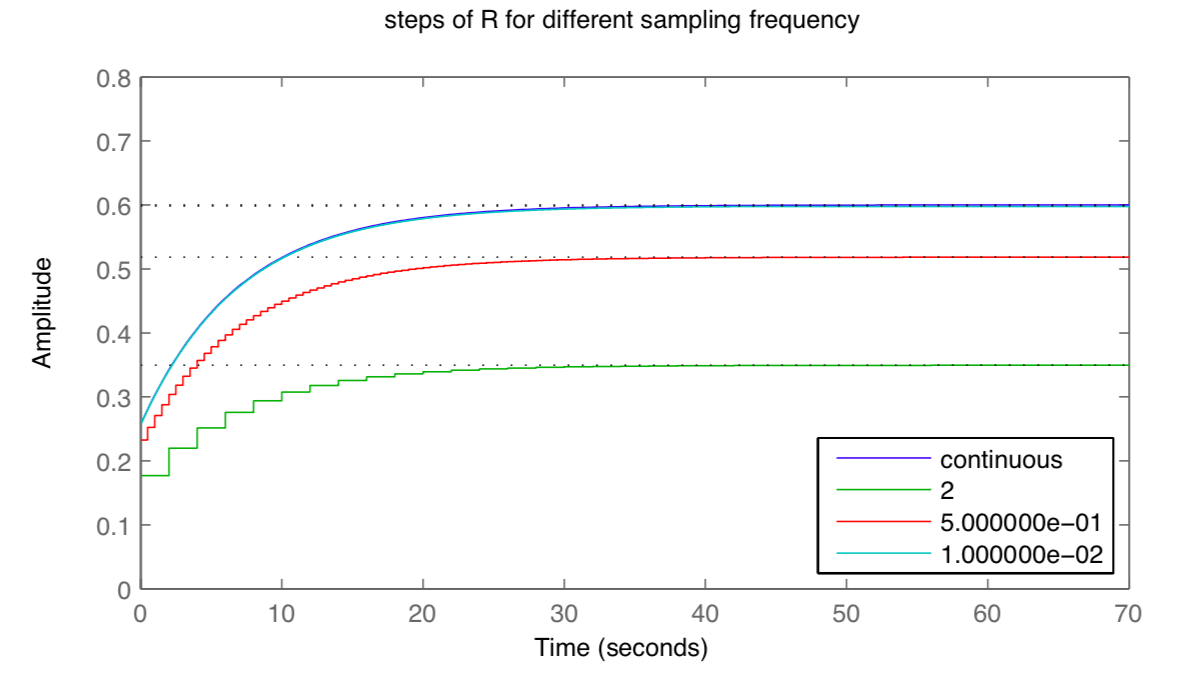
\includegraphics[width=1\linewidth]{images/graph2_1.png}
\caption{Step réponse du régulateur discrétisé}
\label{labo2-1}
\end{figure}

On observe des amplitudes stabilisées différentes selon la fréquence d'échantillonage utilisée dans la fonction c2d. Au plus la période d'échantillonage est petite au plus le comportement du régulateur discrétisé se rapproche du comportement du régulateur continu (en bleu dans le graphique).\\

Ensuite, il faut comparer les 3 systèmes discrets complets au système continu.\\
La transmitance en boucle ouverte du système est :
$$B_{0} = \frac{3}{5}. \frac{1}{s}$$
La transmittance en boucle fermé est égale à :
$$B_{f} = \frac{1}{\frac{5}{3}.s + 1}$$
La graphique suivant montre la step réponse au système continu et aux 3 systèmes discrets.

\begin{figure}[!h]
\center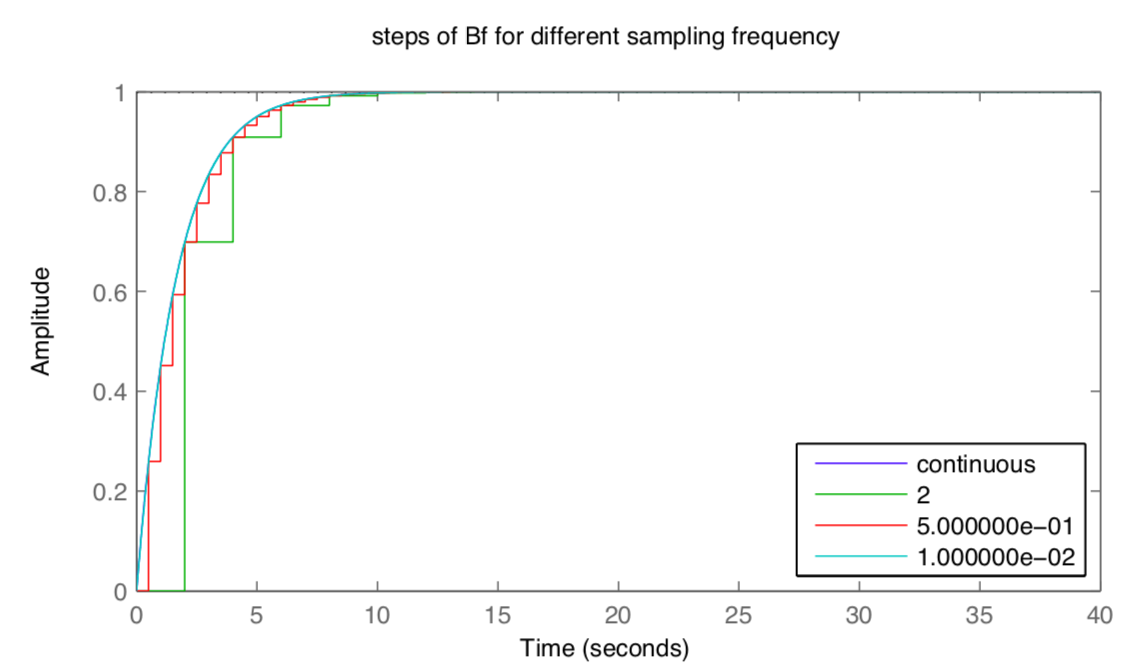
\includegraphics[width=1\linewidth]{images/graph2_2.png}
\caption{Système continu et systèmes discrets}
\label{labo2-2}
\end{figure}
Au plus la période d'échantillonage est petite, au plus la step réponse discrétisé se rapproche de la step réponse continue. 

\newpage
\subsection{Manipulation 3}
Dans cette troisième partie on compare les performances du régulateur continu avec celles des régulateurs discrets :

\begin{figure}[!h]
\center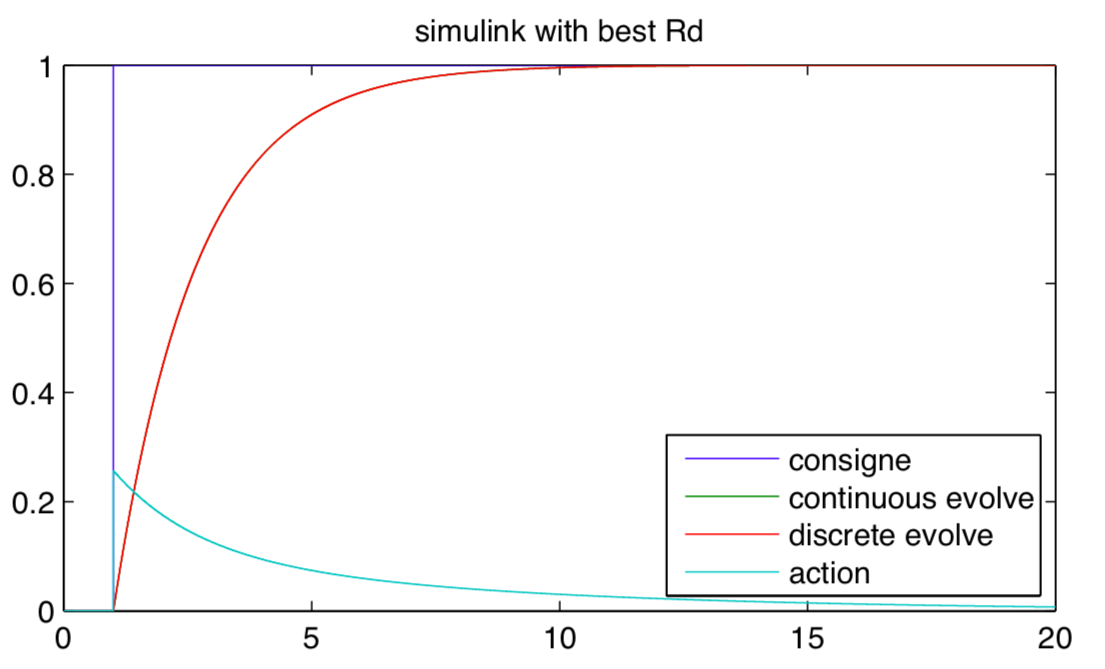
\includegraphics[width=1\linewidth]{images/graph2_3.png}
\label{labo2-3}
\end{figure}
On voit que la réponse du système discrétisé suit bien la consigne.

\subsection{Manipulation 5}

\begin{figure}[!h]
\center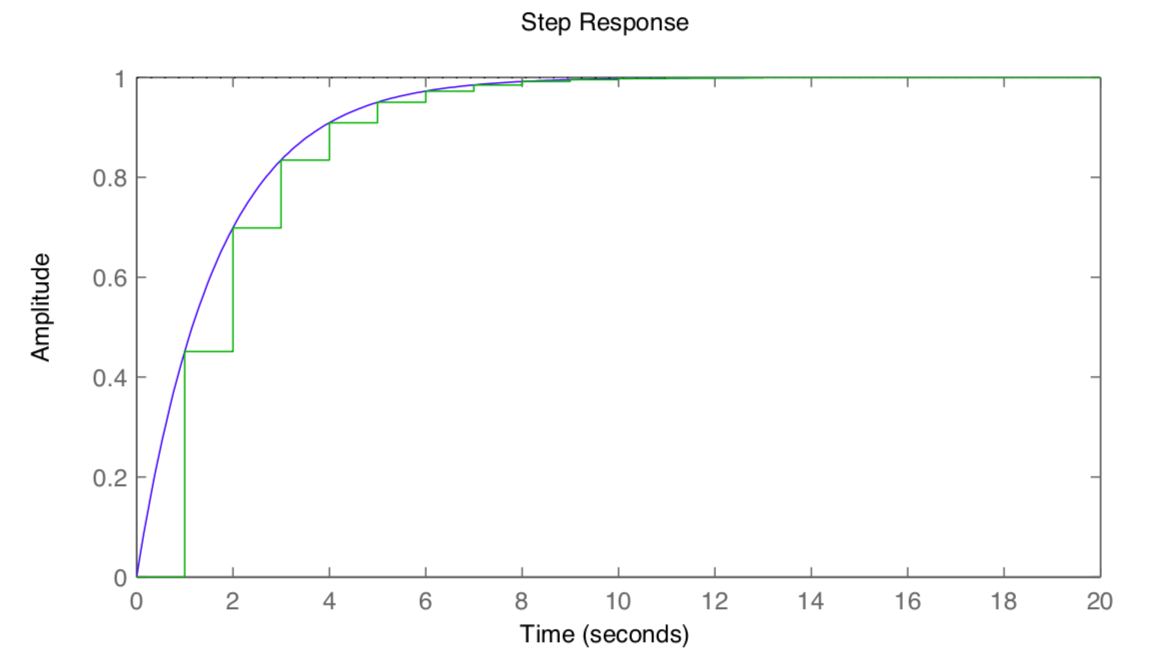
\includegraphics[width=1\linewidth]{images/graph2_4.png}
\label{labo2-4}
\end{figure}

On peut voir ici que la réponse du régulateur discret est bien sur la valeur souhaitée aux instants d'échantillonnages 

\section{Conclusion}

Avec le régulateur discrétisé, on a des dépassements importants tandis qu'avec le vrai régulateur discret malgré que la période d'échantillonnage est importante, aux instants d'échantillonnage on est à nouveau sur la trajectoire.
Cela était donc le but de ces exercices, se rendre compte qu'il faut se méfier quand on fait des synthèses continues et qu'on discrétise.


\section{Codes}
\subsection{s2\_2}
{\footnotesize\begin{verbatim}
clear all;close all;clc
%% 1)
kr = 3/5;

H               = tf([7 1],[3 1 0]);
[zH,pH,kH]      = zpkdata(H,'v');

R               = kr * zpk(pH(2),zH,1/kH);
[zR,pR,kR]      = zpkdata(R,'v');

Bo              = minreal(R*H);
Bf              = minreal(Bo/(1+Bo));

%step(Bf);grid;

%% 2)

h1 = 2;
h2 = 0.5;
h3 = 0.01;
[Rd1,Bfd1]       = s2_getRd(H,h1);
[Rd2,Bfd2]       = s2_getRd(H,h2);
[Rd3,Bfd3]       = s2_getRd(H,h3);

figure
subplot(2,2,1)
rs               = stepplot(R,Rd1,Rd2,Rd3);
title('steps of R for different sampling frequency')
legend('continuous',sprintf('%d',h1),sprintf('%d',h2),sprintf('%d',h3),'Location','southeast')

subplot(2,2,2)
bfs              = stepplot(Bf,Bfd1,Bfd2,Bfd3);
title('steps of Bf for different sampling frequency')
legend('continuous',sprintf('%d',h1),sprintf('%d',h2),sprintf('%d',h3),'Location','southeast')

%% 3)
[zRd,pRd,kRd]   = zpkdata(Rd3,'v');
h  = h3;
sim('s2_sim2.slx');

subplot(2,2,3)
plot(t,yc,t,yr,t,y,t,u)
title('simulink with best Rd')
legend('consigne','continuous evolve','discrete evolve','action','Location','southeast')
%% 4)
h  = h1;
sim('s2_sim2');
subplot(2,2,4)
plot(t,yc,t,yr,t,y,t,u)
title('simulink with best Rd but wrong h')
legend('consigne','continuous evolve','discrete evolve','action','Location','southeast')
%% 5)
h               = 1;
Hd              = c2d(H,h);
[zHd,pHd,kHd]   = zpkdata(Hd,'v');
kRd             = 1-exp((-3/5)*h);
Rd              = kRd * zpk(pHd(2),zHd,1/kHd,h);
[zRd,pRd,kRd]   = zpkdata(Rd,'v');
Bod             = minreal(Hd*Rd);
Bfd             = minreal(Bod/(1+Bod));
rs              = stepplot(R,Rd);
bfs             = stepplot(Bf,Bfd);

\end{verbatim}}


\subsection{s2\_getRd}
{\footnotesize\begin{verbatim}


function [Rd,Bfd] = s2_getRd(H,h)
Hd              = c2d(H,h);
[zHd,pHd,kHd]   = zpkdata(Hd,'v');
kRd             = 1-exp((-3/5)*h);
Rd              = kRd * zpk(pHd(2),zHd,1/kHd,h);
Bod             = minreal(Hd*Rd);
Bfd             = minreal(Bod/(1+Bod));

\end{verbatim}}

